
\section{Empirical Results}\label{sec:experiment}

In this section we present the empirical results obtained from running Hash-join, LIP and LIP-$k$ on several datasets. In Section \ref{sec:dataset}, we present the dataset we used and how we manually apply skewness to generate skewed and adversarial datasets; in Section \ref{sec:time} we present the running time of multiple strategies and discuss their performance; and in Section \ref{sec:ratio} we discuss how $k$ affects the competitive ratio of LIP-$k$ empirically on our dataset.



\subsection{Skewed and Adversarial Datasets}
\label{sec:dataset}
The dataset for testing is obtained from the Star Schema Benchmark \cite{o2009star}. We will hard-code each queries in \cite{o2009star} to measure the join processing time.



\subsection{Execution Time}
\label{sec:time}



\subsection{Competitive Ratio}
\label{sec:ratio}

We ran LIP-$k$ on each skewed dataset we produced and compute the competitive ratio of each LIP-$k$ by taking the maximum of the competitive ratios achieved across all queries in all datasets. The results are depicted in Figure \ref{fig:cr}. 



\begin{figure}
    \centering
  	\subfloat[]{
    	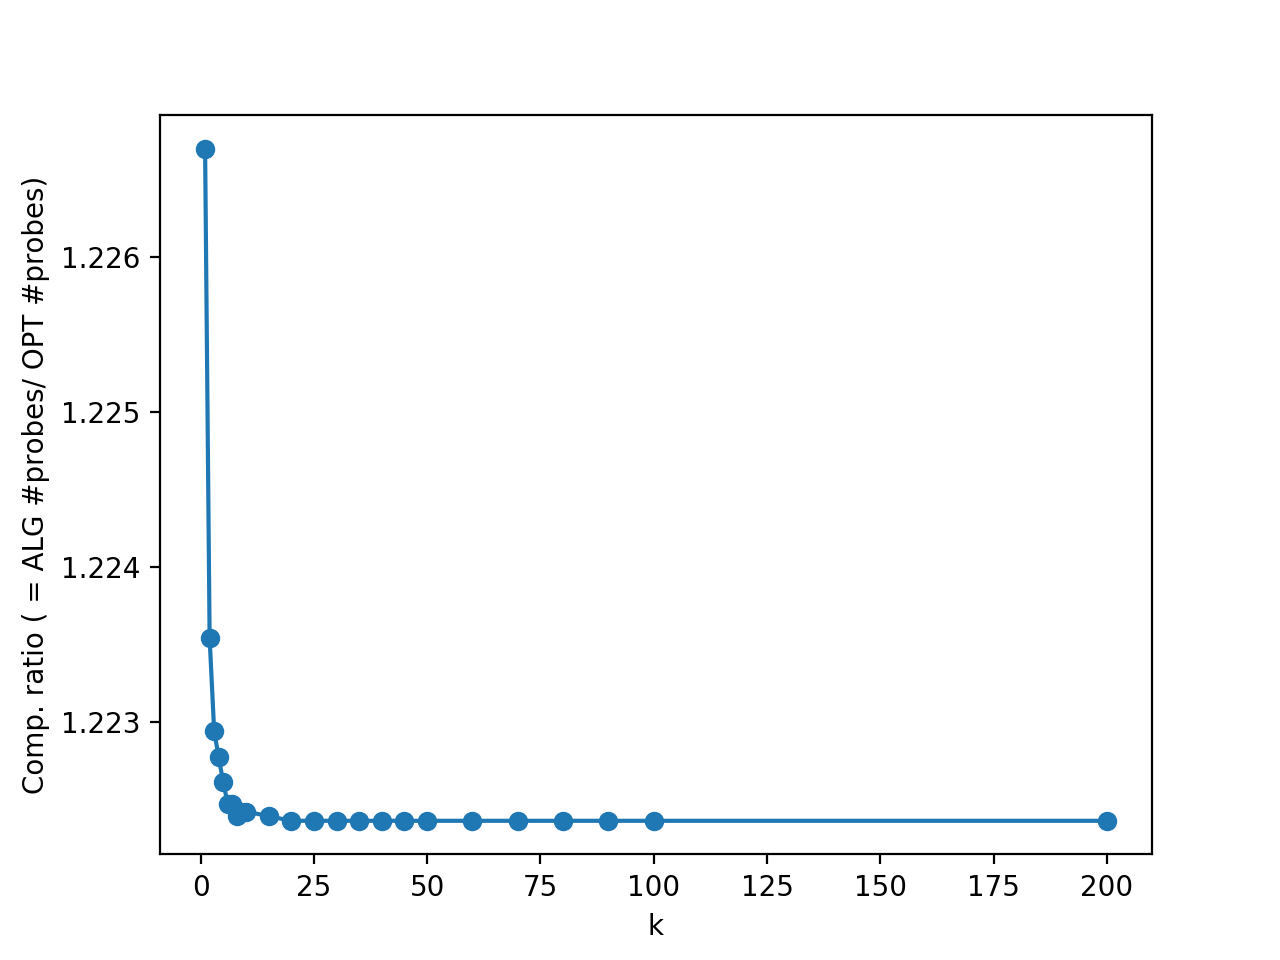
\includegraphics[width=0.43\textwidth,keepaspectratio]{cr-k-uniform}
  	}	
    \quad
    \subfloat[]{
    	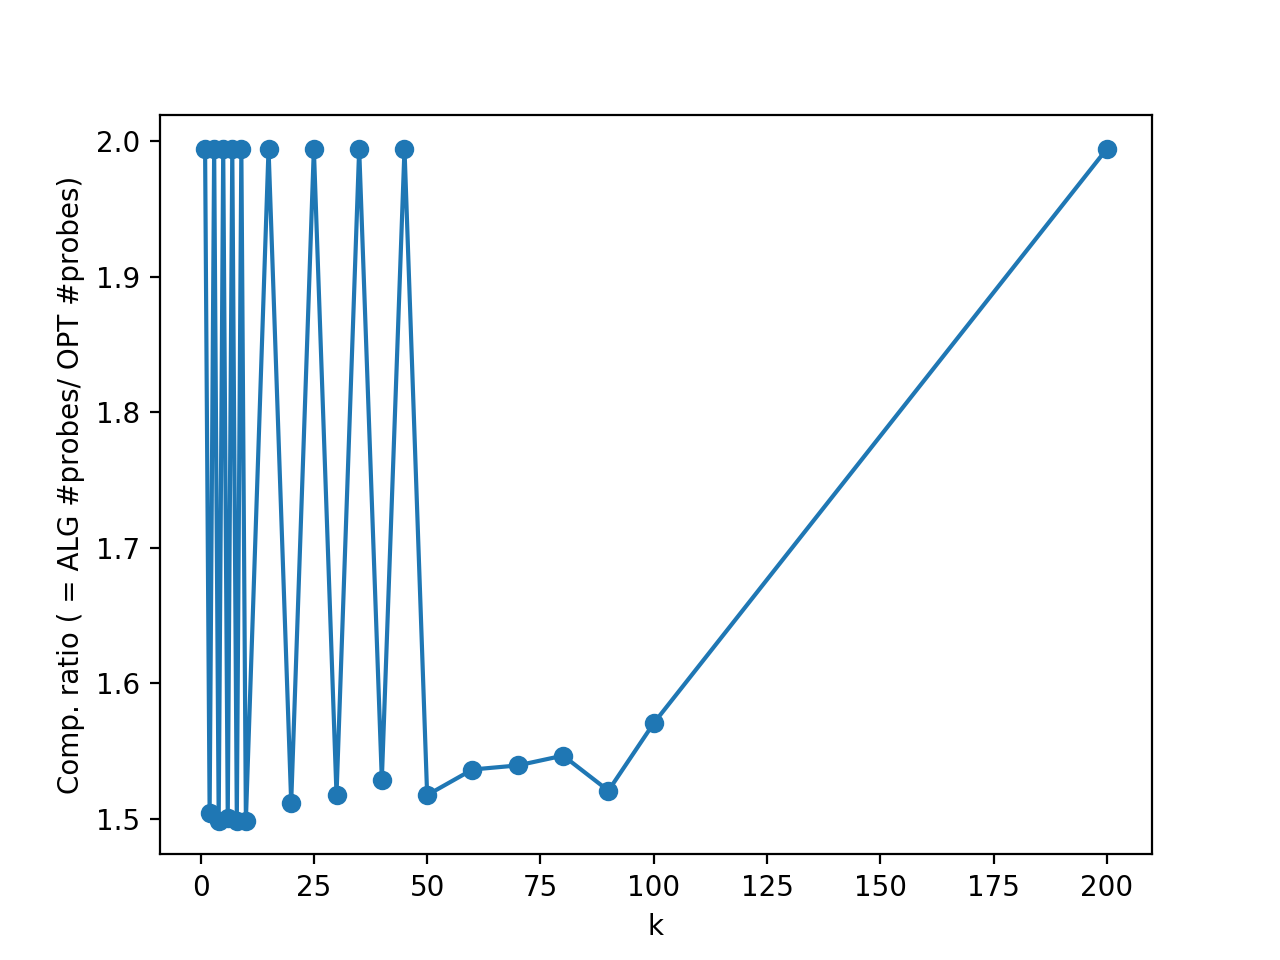
\includegraphics[height=0.32\textwidth,keepaspectratio]{cr-k-skewed}
    }
    \caption{The competitive ratios of LIP-$k$ against different $k$ values. We ran LIP-$k$ on uniform data and skewed (and adversarial) dataset to produce (a) and (b) respectively. The data point at $k = 200$ represents LIP (which is essentially LIP-$\infty$).}
    \label{fig:cr}
\end{figure}

When the keys in the fact table columns are distributed uniformly, the filters need not to react to the local changes. Hence for LIP with higher $k$, it remembers more batches in the uniform data, therefore may produce relatively more accurate estimate of the selectivities than the LIP with lower $k$. Hence the competitive ratio would decrease (slightly) when $k$ increases, as depicted in Figure \ref{fig:cr}.  


Figure \ref{fig:cr} (b) displays how an adversarial dataset can make LIP-$k$ and LIP perform inefficiently. In fact, each LIP-$k$ with even $k$ achieves an approximation ratio less than 2; LIP and LIP-$k$ with odd $k$ achieve an approximation ratio of almost 2 precisely at Query 3.2 in dataset \texttt{date-50-50}. Query 3.2 has two joins, and thus the performance of LIP-$k$ with even $k$ matches the worst case competitive ratio.	

%$k = 1, 2, 3, 4, 5, 10, 15, 20, 25, 30, 35, 40, 45, 50, 60, 70, 80, 90, 100$ on 